\documentclass[tikz]{standalone}

\usepackage{tikz}
\usetikzlibrary{matrix}

\begin{document}
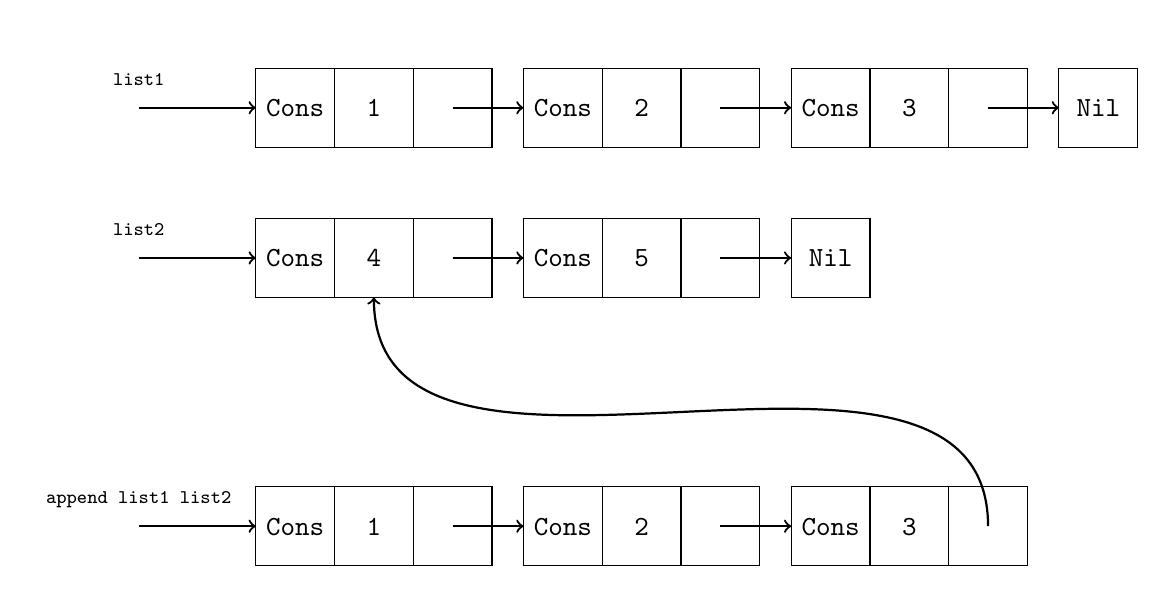
\begin{tikzpicture}[cell/.style={rectangle,draw=black},
space/.style={minimum height=1.5em,matrix of nodes,row sep=-\pgflinewidth,column sep=-\pgflinewidth,column 1/.style={font=\ttfamily}},text depth=0.5ex,text height=2ex,nodes in empty cells]

\tikzset{listarrow/.style={->, thick}}

\matrix (lists) [matrix of nodes,%
   column sep=-\pgflinewidth,%
   row sep=5mm,%
   nodes in empty cells,
   nodes={draw, minimum width=1cm, outer sep=0pt, minimum
     height=1cm, anchor=center}] {
 |[draw=none, label={[label distance=-6mm]\scriptsize \texttt{list1}}]| &[2mm] \texttt{Cons} & \texttt{1} & &[4mm] \texttt{Cons} & \texttt{2} & &[4mm] \texttt{Cons} & \texttt{3} & &[4mm] \texttt{Nil}\\
 |[draw=none, label={[label distance=-6mm]\scriptsize \texttt{list2}}]| &[2mm] \texttt{Cons} & \texttt{4} & &[4mm] \texttt{Cons} & \texttt{5} & &[4mm] \texttt{Nil}\\
 |[draw=none]|\\
 |[draw=none, label={[label distance=-6mm]\scriptsize \texttt{append list1 list2}}]| &[2mm] \texttt{Cons} & \texttt{1} & &[4mm] \texttt{Cons} & \texttt{2} & &[4mm] \texttt{Cons} & \texttt{3} &\\
};

\draw[listarrow] (lists-1-1.center) -- (lists-1-2.west);
\draw[listarrow] (lists-1-4.center) -- (lists-1-5.west);
\draw[listarrow] (lists-1-7.center) -- (lists-1-8.west);
\draw[listarrow] (lists-1-10.center) -- (lists-1-11.west);

\draw[listarrow] (lists-2-1.center) -- (lists-2-2.west);
\draw[listarrow] (lists-2-4.center) -- (lists-2-5.west);
\draw[listarrow] (lists-2-7.center) -- (lists-2-8.west);

\draw[listarrow] (lists-4-1.center) -- (lists-4-2.west);
\draw[listarrow] (lists-4-4.center) -- (lists-4-5.west);
\draw[listarrow] (lists-4-7.center) -- (lists-4-8.west);
\draw[listarrow] (lists-4-10.center) to[out=90,in=270] (lists-2-3.south);

\end{tikzpicture}
\end{document}
